\documentclass[11pt]{article}
\usepackage{icmlko}
\begin{document}

\title{죽은 손잡이 셋을 되살려 보니 셋이 다른 답을 했다}
\author{월드모델 실험실}
\date{노트 427 · 2026년 8월 3일}
\maketitle

\begin{abstract}
노트 426이 규약을 대칭으로 만들면서 방향을 하나 열었다 --- \emph{판으로
죽인 손잡이가 전이에서는 살아 있을 수 있다.} 깊이가 그 첫 예였다(노트 412가
판으로 물렸는데 전이 $+0.029$). 같은 처지가 셋 더 있었고 \textbf{전이 쪽에서
한 번도 안 재 봤다}.

\begin{center}
\begin{tabular}{llrl}
\hline
손잡이 & 판에서 죽은 자리 & 앱 전이 & \\
\hline
\textbf{lr $0.10$} & $+0.0005 \cdot 6/12$ (노트 408) & $\mathbf{+0.0046}$ & $1.000$ \\
\texttt{seq} 축 & $\mathbf{-0.0000} \cdot 7/12$ (노트 415) & $\mathbf{-0.0000}$ & $0.495$ \\
자루 깊이섞기 & $-0.0007 \cdot 2/12$ (노트 409) & $\mathbf{-0.0081}$ & $0.000$ \\
\hline
\end{tabular}
\end{center}

\textbf{셋이 서로 다른 답을 했다.} 하나는 살아 있었고, 하나는 판에서도
전이에서도 \textbf{정확히 아무것도 아니었고}, 하나는 판정이 옳았다.
\textbf{``판으로 죽인 것을 전이에서 다시 본다''가 만능이 아니라는 것을
같은 실험이 같이 보여 준다.}
\end{abstract}

\section{lr $0.10$ --- 살아 있었다 · 채택}

노트 408은 $K{=}8$ 쓸기에서 $+0.0028$ 이던 것이 $K{=}32$ 관문에서
$+0.0005 \cdot 6/12$ 로 녹는 것을 보고 유지했다. 그때 잰 것은 판뿐이었다.

\begin{center}
\begin{tabular}{lr}
\hline
비게임 앱 전이 & $+0.0046$ \ $[+0.0022, +0.0071]$ \ $1.000$ \\
KR 만화 전이 & $+0.0121$ \ $[-0.0036, +0.0273]$ \ $0.949$ \\
판 (깊이 12 재관문) & $-0.0005 \pm 0.0020 \cdot 5/12$ \\
\hline
\end{tabular}
\end{center}

노트 426의 규약이 그대로 걸린다 --- 안 본 도메인 \textbf{둘이 같은 부호}이고
앱 쪽 구간이 0 을 안 물며, 판 손해 $0.0005$ 가 $2\times$짝SD($0.0040$) 안이다.
\textbf{채택했다.}

그런데 실제 자료에서는 판이 \textbf{오른다} --- 씨앗 12평균
$0.4714 \to \mathbf{0.4742 \pm 0.0007}$. 아이돌 하나가 $+0.0516$ 이다.
관문이 또 보수적이었다(노트 406과 같은 자리).

\section{\texttt{seq} --- 정말 아무것도 아니었다}

노트 415가 \texttt{seq} 를 판 $-0.0000 \cdot 7/12$ 로 닫으면서 ``애니엔
$+0.0103$ 인데 도서 $-0.0434$ 가 지운다''고 적었다. \textbf{전이에서도
$-0.0000$ 이다}($[-0.0041, +0.0044]$, $0.495$).

판에서 $0$, 전이에서 $0$ --- 이만큼 깨끗한 무효는 드물다. \textbf{속편
여부는 이 판에서 쓸 축이 아니다}, 노트 181이 애니 안에서 잰 신호가 아무리
또렷했어도. 닫는다.

\section{자루 깊이섞기 --- 판정이 옳았다}

노트 409가 판 $-0.0007 \cdot 2/12$ 로 물렸고, 그때 ``용량은 자루로 못
쪼갠다''고 적었다. 전이에서도 $-0.0081$ 로 \textbf{확실히 잃는다}
($[-0.0111, -0.0052]$, $0.000$).

\textbf{판과 목표가 같은 말을 한 첫 손잡이다.} 노트 420·426이 둘이 갈라지는
자리만 다뤘는데, 갈라지지 않는 자리도 있다는 것을 이것이 보인다.

\section{남은 것}

\begin{tabular}{lp{7.0cm}}
\hline
$K$ 와 축 묶음 & 아직 전이에서 안 봤다. 남은 ``죽은 손잡이''는 그 둘 \\
lr 을 더 & $0.10$ 이 사는데 $0.14$·$0.20$ 은 안 재 봤다. 깊이처럼 포화점이
있을 것이다 \\
관문의 보수성 & 깊이(노트 406)·lr(여기) 둘 다 실제 자료가 관문보다 좋다.
\textbf{되뽑기 관문이 체계적으로 낮게 잰다}면 그것 자체가 잴 거리다 \\
\hline
\end{tabular}

\begin{figure}[h]
\centering
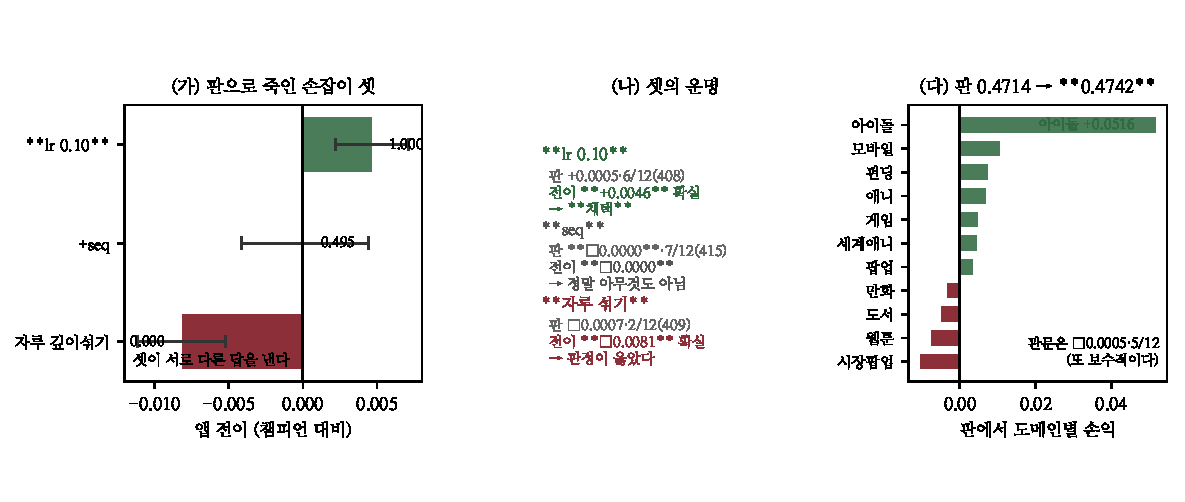
\includegraphics[width=\textwidth]{figs/fig427.pdf}
\caption{(가) 셋의 앱 전이. (나) 셋의 운명이 다 다르다. (다) 채택 뒤
판 $0.4714 \to 0.4742$ --- 아이돌이 끌어올린다.}
\end{figure}

\end{document}
